%Note: Lad vaere med at skrive e.g. i hver anden saetning.

As computers are becoming a more integral part of our lives, they are becoming more integrated with out educational system as well.
Different educational methods are supported by different information communication systems called e-learning systems.
These observation has lead us to investigate how the method of our university can be implemented into the e-learning system being used at our university.

This project is conducted as a multi-project, which means that sub-groups will be working on sub-projects and these groups must work together to complete the whole project.
This chapter of the report is shared among every sub-group and contains the exact same content.
In this chapter ``we'' refers to all 14 members of the multi-project.

\section{E-Learning}
\label{sec:e-learning}
The term e-learning covers all forms of electronically supported learning. 
E-learning is often associated with distance learning and out-of-classroom teaching, but can also be used to support traditional teaching in class rooms. 
In short e-learning is defined as learning that is facilitated and supported via \emph{ICT} (Information and Communications Technology). 
The cooperation between the teachers and students and among the students themselves can similarly be partially or completely conducted via ICT~\cite{def-e-learning1}~\cite{def-e-learning2}.

E-learning is growing in popularity; it was noted in 2007 that 20\% of all higher education students in the U.S. were taking at least one course online, and that does not include the courses, which makes use of some form of e-learning.	
At Aalborg University e-learning is employed in a variety of forms. 
There are fully online courses taught by The Institute of Problem Based Learning (PBL)~\cite{mpbl}, and regular courses that make use of online quizes as a method of teaching.

\subsection{Learning Management Systems}
\label{sub:lms}
E-learning is often conducted through the use of a Learning Management System (LMS). 
An LMS is loosely defined as a software system, which administrates, tracks, and reports teaching. 
It is considered robust if it contains the following functionality~\citep{Ellis09}:

\begin{itemize}
	\item Has centralized and automated administration
	\item Uses self-service and self-guided service
	\item Is able to assemble and deliver learning content rapidly
	\item Consolidates teaching activities on a scalable web-based platform
	\item Supports portability and standards
	\item Has the ability personalize- and reuse content
\end{itemize}

LMSs have many forms each catered to a specific target groups. 
%As an example a LMS by a company to manage internal training would have different requirements than one used at a University. 
The general characteristics of a LMS are~\citep{Kerschenbaum}

\begin{itemize}
	\item Student registration and administration
	\item Management of teaching events such as scheduling and tracking
	\item Management of curriculums and obtained qualifications
	\item Management of skills and competencies (mostly for corporate use)
	\item Reporting of grades and approved assignments
	\item Management of	a teaching records
	\item The ability to produce and share material relevant to courses

%	\item Management functionality for users, roles, courses, instructors, facilities, etc.
%	\item A course calendar
%	\item Communication and notification functionality for students
%	\item Assessment and management of tests both before and after they are conducted
%	\item The ability to display scores and transcripts for students 
%	\item The ability to grade coursework and manage course rosters, including course wait lists
%	\item Support for partially or fully online courses
\end{itemize}

The purpose of a LMS is to handle and administrate all study related activities at a learning institution.%, and as e-learning is defined in section~\ref{sec:e-learning} as learning supported or facilitated through ICT, LMSs and e-learning are closely related.

Moodle (\emph{Modular Object-Oriented Dynamic Learning Environment}) \citep{moodle} is currently the primary e-learning platform at AAU. 
Its main purpose is to allow lecturers to share course-relevant material with students and to serve as a calendar service containing dates of lectures, meetings etc. 
The problem is that Moodle does not support PBL, which is the learning method used at AAU.

\subsection{The Aalborg PBL Model}
\label{sub:aaupbl}
The Aalborg PBL model is a term coined to describe Aalborg University's problem and project based learning model. 
It originates from the philosophy of the university's faculty. 
They were interested in giving the students an active role in obtaining knowledge, as opposed to the lecture based learning method used at many universities.
Furthermore, they wanted to give the faculty an more active role in the students' learning experience than what the lecture setting provided. 
From this the Aalborg PBL Model was developed. 
This section is based on~\citep{Barge10}.

The Aalborg PBL Model has six terms, which describe the basic concept of the model:

\begin{itemize}
	\item \textbf{Problem} - A written formulation of a problem, which can be theoretical or practical. 
	It is sparked by the students' curiosity. 
	The problem serves as the starting point for the students' learning and puts them into a concrete context. 
	A problem must be exemplary and can contain interdisciplinary approaches	in both the analysis and solving phase.
	\item \textbf{Project} - A task which requires an analysis of a new and complex problem. It must be planned and managed, as it might potentially affect people's surroundings, organization, knowledge, and attitude to life, and it must be completed on time. Projects are diverse in regards to scope and definition.
	\item \textbf{Exemplarity} - The problem a project is concerned with must be exemplary, that is it must relatable to a specific practical, scientific, or technical domain.
	\item \textbf{Team} - A team is a group working together on a project. 
	Their cooperation on the different aspects of a successfully completed project is essential to the approach of learning.
	\item \textbf{Supervisor} - A role usually held by faculty members, the supervisor serves a resource for a group of students working on a project to rely on for help and feedback. 
	The supervisor is only assigned to a particular group for the duration of the project. 
	\item \textbf{Courses} - Courses are given to the students, which fit within the theme for a semester. 
	Courses provide knowledge that is either relevant to the students project or field of study.
\end{itemize}

The Aalborg PBL Model consists up of six core principles, which outline the students' learning process.
\begin{itemize}
	\item \textbf{Problem orientation} - A problem relevant to the students' field of study that serves as the basis for their learning process.
	\item \textbf{Project organization} - The project is the medium through which the students address the problem and achieve the knowledge outlined by the curriculum.
	\item \textbf{Integration of theory and practice} - The curriculum and staff at the university are responsible for teaching the students to connect their project work to broader theoretical knowledge.
	\item \textbf{Participant direction} - Students define their problem and make decisions relevant to the completion of the project themselves.
	\item \textbf{Team-based approach} - Most of the students' project related work is conducted in groups of three or more students.
	\item \textbf{Collaboration and feedback} - Peer and supervisor critique is used continuously throughout a project to improve the students' work.
	The aim is for the students gain the skills of collaboration, feedback, and reflection by following the PBL model. 
\end{itemize}

\section{Moodle}
Moodle is an e-learning platform for producing dynamic web sites for courses. 
Moodle was originally developed by Martin Dougiamas in 2002 and is released under an open source license (GPLv3+) \citep{gpl}. 
It is currently maintained by a group of core developers. 
Due to its modular design, the functionality of Moodle can be extended with plugins developed by the Moodle community.

Moodle is build up around the concept of courses, and most activities in Moodle are centered around them. 
Courses can be divided into categories, and topics, resources, activities, and blocks can be added to them. 
Topics is an integrated part of courses, and resources can be links to external sources or uploaded files. 
Both these elements are an integrated part of courses. 
Activities and blocks are plugins, which can be added to a course to provide additional functionality. 
An activity is added by placing a link on a page, where the activities functionality lies. 
A block can be shown visually on the course page~\citep{moodleStructural}.
An example of a Moodle course page can be seen in Figure~\ref{fig:MoodleCourse}

\begin{figure}
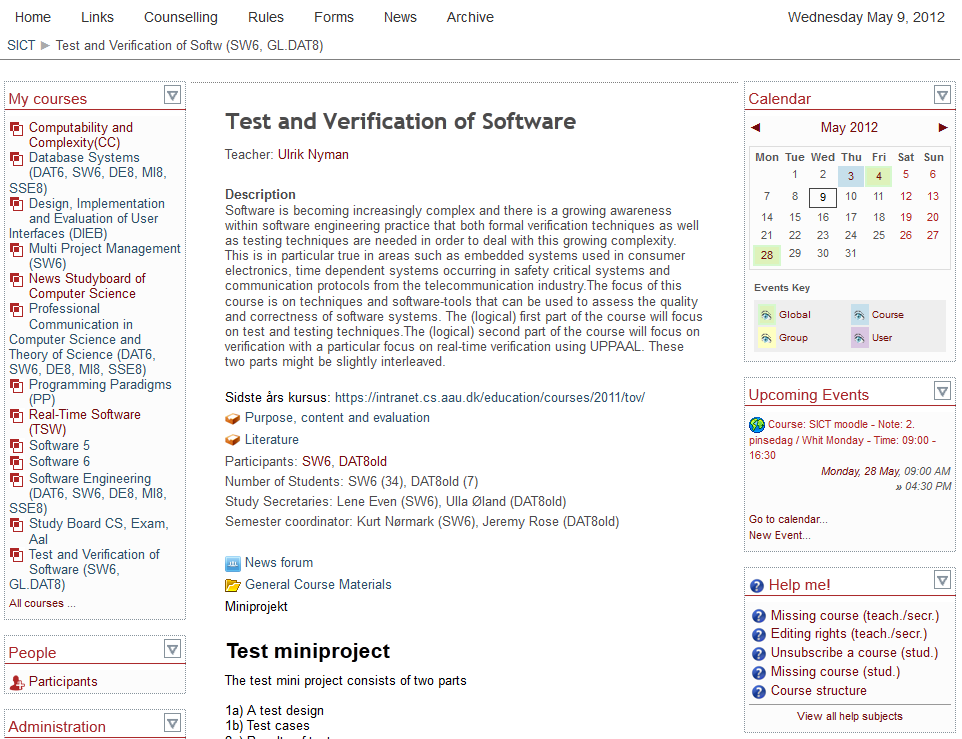
\includegraphics[width=\textwidth]{moodle_page}
\caption{A Moodle course page}
\label{fig:MoodleCourse}
\end{figure}

However, as Moodle is built up around courses it does not provide much functionality to support the way that students work on projects at AAU. 
The students collaborate in groups in order to solve realistic problems, which is also known as \emph{problem-based learning}, or more specific, the \emph{Aalborg PBL Model} \citep{pbl}. This serves as the motivation for the following problem definition.

\section{Problem Definition}
\label{sec:problemDef}
%The work method used at AAU does not synergize well with Moodle NOTE: synergize er ikke et ord. Synergy er et ord, men et navneord
Moodle does not fully support the work method used at AAU. 
Moodle is built up strictly around courses, and does not contain the concept of project groups. 
To accommodate for this students must use different tools for project group work.
This report will be concerned with how to implement support for the Aalborg PBL Model in Moodle. 
This involves researching other systems than Moodle for how they accommodate project groups, and conducting interviews with both members of the faculty and students to gather requirements for such an extension to Moodle.